\documentclass[twoside]{book}

% Packages required by doxygen
\usepackage{fixltx2e}
\usepackage{calc}
\usepackage{doxygen}
\usepackage[export]{adjustbox} % also loads graphicx
\usepackage{graphicx}
\usepackage[utf8]{inputenc}
\usepackage{makeidx}
\usepackage{multicol}
\usepackage{multirow}
\PassOptionsToPackage{warn}{textcomp}
\usepackage{textcomp}
\usepackage[nointegrals]{wasysym}
\usepackage[table]{xcolor}

% Font selection
\usepackage[T1]{fontenc}
\usepackage[scaled=.90]{helvet}
\usepackage{courier}
\usepackage{amssymb}
\usepackage{sectsty}
\renewcommand{\familydefault}{\sfdefault}
\allsectionsfont{%
  \fontseries{bc}\selectfont%
  \color{darkgray}%
}
\renewcommand{\DoxyLabelFont}{%
  \fontseries{bc}\selectfont%
  \color{darkgray}%
}
\newcommand{\+}{\discretionary{\mbox{\scriptsize$\hookleftarrow$}}{}{}}

% Page & text layout
\usepackage{geometry}
\geometry{%
  a4paper,%
  top=2.5cm,%
  bottom=2.5cm,%
  left=2.5cm,%
  right=2.5cm%
}
\tolerance=750
\hfuzz=15pt
\hbadness=750
\setlength{\emergencystretch}{15pt}
\setlength{\parindent}{0cm}
\setlength{\parskip}{0.2cm}
\makeatletter
\renewcommand{\paragraph}{%
  \@startsection{paragraph}{4}{0ex}{-1.0ex}{1.0ex}{%
    \normalfont\normalsize\bfseries\SS@parafont%
  }%
}
\renewcommand{\subparagraph}{%
  \@startsection{subparagraph}{5}{0ex}{-1.0ex}{1.0ex}{%
    \normalfont\normalsize\bfseries\SS@subparafont%
  }%
}
\makeatother

% Headers & footers
\usepackage{fancyhdr}
\pagestyle{fancyplain}
\fancyhead[LE]{\fancyplain{}{\bfseries\thepage}}
\fancyhead[CE]{\fancyplain{}{}}
\fancyhead[RE]{\fancyplain{}{\bfseries\leftmark}}
\fancyhead[LO]{\fancyplain{}{\bfseries\rightmark}}
\fancyhead[CO]{\fancyplain{}{}}
\fancyhead[RO]{\fancyplain{}{\bfseries\thepage}}
\fancyfoot[LE]{\fancyplain{}{}}
\fancyfoot[CE]{\fancyplain{}{}}
\fancyfoot[RE]{\fancyplain{}{\bfseries\scriptsize Generated on Mon Jun 27 2016 17\+:56\+:35 for Zato Client by Doxygen }}
\fancyfoot[LO]{\fancyplain{}{\bfseries\scriptsize Generated on Mon Jun 27 2016 17\+:56\+:35 for Zato Client by Doxygen }}
\fancyfoot[CO]{\fancyplain{}{}}
\fancyfoot[RO]{\fancyplain{}{}}
\renewcommand{\footrulewidth}{0.4pt}
\renewcommand{\chaptermark}[1]{%
  \markboth{#1}{}%
}
\renewcommand{\sectionmark}[1]{%
  \markright{\thesection\ #1}%
}

% Indices & bibliography
\usepackage{natbib}
\usepackage[titles]{tocloft}
\setcounter{tocdepth}{3}
\setcounter{secnumdepth}{5}
\makeindex

% Hyperlinks (required, but should be loaded last)
\usepackage{ifpdf}
\ifpdf
  \usepackage[pdftex,pagebackref=true]{hyperref}
\else
  \usepackage[ps2pdf,pagebackref=true]{hyperref}
\fi
\hypersetup{%
  colorlinks=true,%
  linkcolor=blue,%
  citecolor=blue,%
  unicode%
}

% Custom commands
\newcommand{\clearemptydoublepage}{%
  \newpage{\pagestyle{empty}\cleardoublepage}%
}


%===== C O N T E N T S =====

\begin{document}

% Titlepage & ToC
\hypersetup{pageanchor=false,
             bookmarks=true,
             bookmarksnumbered=true,
             pdfencoding=unicode
            }
\pagenumbering{roman}
\begin{titlepage}
\vspace*{7cm}
\begin{center}%
{\Large Zato Client }\\
\vspace*{1cm}
{\large Generated by Doxygen 1.8.10}\\
\vspace*{0.5cm}
{\small Mon Jun 27 2016 17:56:35}\\
\end{center}
\end{titlepage}
\clearemptydoublepage
\tableofcontents
\clearemptydoublepage
\pagenumbering{arabic}
\hypersetup{pageanchor=true}

%--- Begin generated contents ---
\chapter{Namespace Index}
\section{Namespace List}
Here is a list of all documented namespaces with brief descriptions\+:\begin{DoxyCompactList}
\item\contentsline{section}{\hyperlink{namespacezato}{zato} }{\pageref{namespacezato}}{}
\end{DoxyCompactList}

\chapter{Hierarchical Index}
\section{Class Hierarchy}
This inheritance list is sorted roughly, but not completely, alphabetically\+:\begin{DoxyCompactList}
\item \contentsline{section}{zato\textbackslash{}Debug}{\pageref{classzato_1_1_debug}}{}
\item Exception\begin{DoxyCompactList}
\item \contentsline{section}{zato\textbackslash{}Exceptions\textbackslash{}Api\+Response\+Exception}{\pageref{classzato_1_1_exceptions_1_1_api_response_exception}}{}
\item \contentsline{section}{zato\textbackslash{}Exceptions\textbackslash{}Auth\+Exception}{\pageref{classzato_1_1_exceptions_1_1_auth_exception}}{}
\end{DoxyCompactList}
\item \contentsline{section}{zato\textbackslash{}Http}{\pageref{classzato_1_1_http}}{}
\item \contentsline{section}{zato\textbackslash{}Resources\textbackslash{}Resource\+Abstract}{\pageref{classzato_1_1_resources_1_1_resource_abstract}}{}
\begin{DoxyCompactList}
\item \contentsline{section}{zato\textbackslash{}Resources\textbackslash{}Core\textbackslash{}Ping}{\pageref{classzato_1_1_resources_1_1_core_1_1_ping}}{}
\item \contentsline{section}{zato\textbackslash{}Resources\textbackslash{}Services\textbackslash{}Invoke}{\pageref{classzato_1_1_resources_1_1_services_1_1_invoke}}{}
\end{DoxyCompactList}
\item \contentsline{section}{zato\textbackslash{}Zato\+Client}{\pageref{classzato_1_1_zato_client}}{}
\end{DoxyCompactList}

\chapter{Class Index}
\section{Class List}
Here are the classes, structs, unions and interfaces with brief descriptions\+:\begin{DoxyCompactList}
\item\contentsline{section}{\hyperlink{classzato_1_1_exceptions_1_1_api_response_exception}{zato\textbackslash{}\+Exceptions\textbackslash{}\+Api\+Response\+Exception} }{\pageref{classzato_1_1_exceptions_1_1_api_response_exception}}{}
\item\contentsline{section}{\hyperlink{classzato_1_1_exceptions_1_1_auth_exception}{zato\textbackslash{}\+Exceptions\textbackslash{}\+Auth\+Exception} }{\pageref{classzato_1_1_exceptions_1_1_auth_exception}}{}
\item\contentsline{section}{\hyperlink{classzato_1_1_debug}{zato\textbackslash{}\+Debug} }{\pageref{classzato_1_1_debug}}{}
\item\contentsline{section}{\hyperlink{classzato_1_1_http}{zato\textbackslash{}\+Http} }{\pageref{classzato_1_1_http}}{}
\item\contentsline{section}{\hyperlink{classzato_1_1_resources_1_1_services_1_1_invoke}{zato\textbackslash{}\+Resources\textbackslash{}\+Services\textbackslash{}\+Invoke} }{\pageref{classzato_1_1_resources_1_1_services_1_1_invoke}}{}
\item\contentsline{section}{\hyperlink{classzato_1_1_resources_1_1_core_1_1_ping}{zato\textbackslash{}\+Resources\textbackslash{}\+Core\textbackslash{}\+Ping} }{\pageref{classzato_1_1_resources_1_1_core_1_1_ping}}{}
\item\contentsline{section}{\hyperlink{classzato_1_1_resources_1_1_resource_abstract}{zato\textbackslash{}\+Resources\textbackslash{}\+Resource\+Abstract} }{\pageref{classzato_1_1_resources_1_1_resource_abstract}}{}
\item\contentsline{section}{\hyperlink{classzato_1_1_zato_client}{zato\textbackslash{}\+Zato\+Client} }{\pageref{classzato_1_1_zato_client}}{}
\end{DoxyCompactList}

\chapter{Namespace Documentation}
\hypertarget{namespacezato}{}\section{zato Namespace Reference}
\label{namespacezato}\index{zato@{zato}}
\subsection*{Classes}
\begin{DoxyCompactItemize}
\item 
class \hyperlink{classzato_1_1_debug}{Debug}
\item 
class \hyperlink{classzato_1_1_http}{Http}
\item 
class \hyperlink{classzato_1_1_zato_client}{Zato\+Client}
\end{DoxyCompactItemize}


\subsection{Detailed Description}
Class Api\+Response\+Exception

Auth\+Exception is for auth specific errors  
\chapter{Class Documentation}
\hypertarget{classzato_1_1_exceptions_1_1_api_response_exception}{}\section{zato\textbackslash{}Exceptions\textbackslash{}Api\+Response\+Exception Class Reference}
\label{classzato_1_1_exceptions_1_1_api_response_exception}\index{zato\textbackslash{}\+Exceptions\textbackslash{}\+Api\+Response\+Exception@{zato\textbackslash{}\+Exceptions\textbackslash{}\+Api\+Response\+Exception}}
Inheritance diagram for zato\textbackslash{}Exceptions\textbackslash{}Api\+Response\+Exception\+:\begin{figure}[H]
\begin{center}
\leavevmode
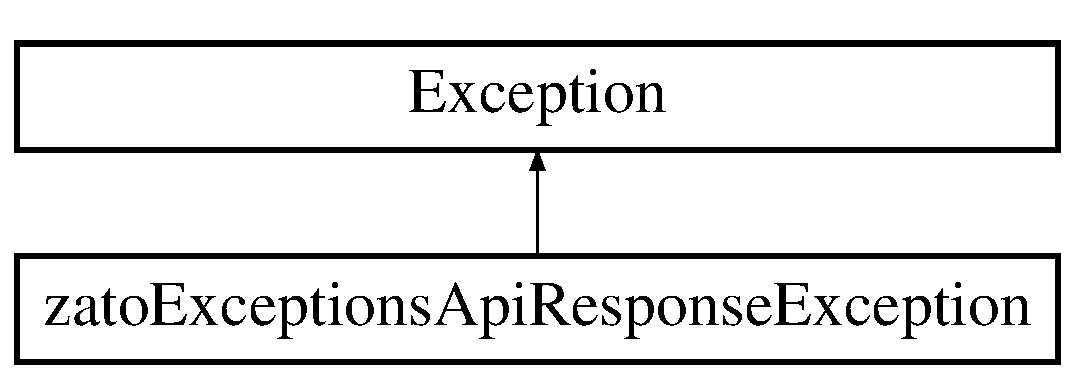
\includegraphics[height=2.000000cm]{classzato_1_1_exceptions_1_1_api_response_exception}
\end{center}
\end{figure}
\subsection*{Public Member Functions}
\begin{DoxyCompactItemize}
\item 
\hypertarget{classzato_1_1_exceptions_1_1_api_response_exception_a5dd842976151781e2459cf1d91453c2c}{}{\bfseries \+\_\+\+\_\+construct} (Request\+Exception \$e)\label{classzato_1_1_exceptions_1_1_api_response_exception_a5dd842976151781e2459cf1d91453c2c}

\item 
\hypertarget{classzato_1_1_exceptions_1_1_api_response_exception_a512812fe54b1ef915ab73f34c9b6ba03}{}{\bfseries get\+Error\+Details} ()\label{classzato_1_1_exceptions_1_1_api_response_exception_a512812fe54b1ef915ab73f34c9b6ba03}

\end{DoxyCompactItemize}
\subsection*{Protected Attributes}
\begin{DoxyCompactItemize}
\item 
\hypertarget{classzato_1_1_exceptions_1_1_api_response_exception_a471c7b012a2c77c1503085663c13732e}{}{\bfseries \$error\+Details} = \mbox{[}$\,$\mbox{]}\label{classzato_1_1_exceptions_1_1_api_response_exception_a471c7b012a2c77c1503085663c13732e}

\end{DoxyCompactItemize}


The documentation for this class was generated from the following file\+:\begin{DoxyCompactItemize}
\item 
src/zato/\+Exceptions/Api\+Response\+Exception.\+php\end{DoxyCompactItemize}

\hypertarget{classzato_1_1_exceptions_1_1_auth_exception}{}\section{zato\textbackslash{}Exceptions\textbackslash{}Auth\+Exception Class Reference}
\label{classzato_1_1_exceptions_1_1_auth_exception}\index{zato\textbackslash{}\+Exceptions\textbackslash{}\+Auth\+Exception@{zato\textbackslash{}\+Exceptions\textbackslash{}\+Auth\+Exception}}
Inheritance diagram for zato\textbackslash{}Exceptions\textbackslash{}Auth\+Exception\+:\begin{figure}[H]
\begin{center}
\leavevmode
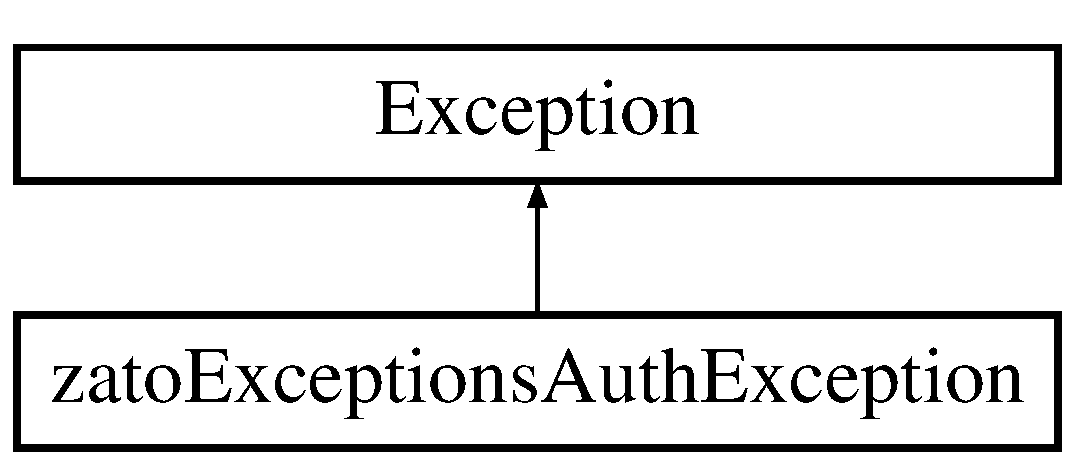
\includegraphics[height=2.000000cm]{classzato_1_1_exceptions_1_1_auth_exception}
\end{center}
\end{figure}


The documentation for this class was generated from the following file\+:\begin{DoxyCompactItemize}
\item 
src/zato/\+Exceptions/Auth\+Exception.\+php\end{DoxyCompactItemize}

\hypertarget{classzato_1_1_debug}{}\section{zato\textbackslash{}Debug Class Reference}
\label{classzato_1_1_debug}\index{zato\textbackslash{}\+Debug@{zato\textbackslash{}\+Debug}}
\subsection*{Public Member Functions}
\begin{DoxyCompactItemize}
\item 
\hyperlink{classzato_1_1_debug_a01ed0dc4c3e81c721525f6279b9b8011}{\+\_\+\+\_\+to\+String} ()
\end{DoxyCompactItemize}
\subsection*{Public Attributes}
\begin{DoxyCompactItemize}
\item 
\hypertarget{classzato_1_1_debug_abd0eadf46c81fa5fb3bf8e3f21bfce4f}{}{\bfseries \$last\+Request\+Body}\label{classzato_1_1_debug_abd0eadf46c81fa5fb3bf8e3f21bfce4f}

\item 
\hypertarget{classzato_1_1_debug_ae38231e8bff154b3375749da4d89ce79}{}{\bfseries \$last\+Request\+Headers}\label{classzato_1_1_debug_ae38231e8bff154b3375749da4d89ce79}

\item 
\hypertarget{classzato_1_1_debug_a43220704abbc5503c3cee9ff854051a3}{}{\bfseries \$last\+Response\+Code}\label{classzato_1_1_debug_a43220704abbc5503c3cee9ff854051a3}

\item 
\hypertarget{classzato_1_1_debug_ae506058db00562d214b7961599a40fe6}{}{\bfseries \$last\+Response\+Headers}\label{classzato_1_1_debug_ae506058db00562d214b7961599a40fe6}

\item 
\hypertarget{classzato_1_1_debug_a1d8f7078a449b05b16335771c8807612}{}{\bfseries \$last\+Response\+Error}\label{classzato_1_1_debug_a1d8f7078a449b05b16335771c8807612}

\end{DoxyCompactItemize}


\subsection{Detailed Description}
\hyperlink{classzato_1_1_debug}{Debug} helper class 

\subsection{Member Function Documentation}
\hypertarget{classzato_1_1_debug_a01ed0dc4c3e81c721525f6279b9b8011}{}\index{zato\+::\+Debug@{zato\+::\+Debug}!\+\_\+\+\_\+to\+String@{\+\_\+\+\_\+to\+String}}
\index{\+\_\+\+\_\+to\+String@{\+\_\+\+\_\+to\+String}!zato\+::\+Debug@{zato\+::\+Debug}}
\subsubsection[{\+\_\+\+\_\+to\+String()}]{\setlength{\rightskip}{0pt plus 5cm}zato\textbackslash{}\+Debug\+::\+\_\+\+\_\+to\+String (
\begin{DoxyParamCaption}
{}
\end{DoxyParamCaption}
)}\label{classzato_1_1_debug_a01ed0dc4c3e81c721525f6279b9b8011}
\begin{DoxyReturn}{Returns}
string 
\end{DoxyReturn}


The documentation for this class was generated from the following file\+:\begin{DoxyCompactItemize}
\item 
src/zato/Debug.\+php\end{DoxyCompactItemize}

\hypertarget{classzato_1_1_http}{}\section{zato\textbackslash{}Http Class Reference}
\label{classzato_1_1_http}\index{zato\textbackslash{}\+Http@{zato\textbackslash{}\+Http}}
\subsection*{Static Public Member Functions}
\begin{DoxyCompactItemize}
\item 
static \hyperlink{classzato_1_1_http_ab8da8edaebf17ce03a9c8cc99fe19195}{send} (\hyperlink{classzato_1_1_zato_client}{Zato\+Client} \$client, \$end\+Point, \$options=\mbox{[}$\,$\mbox{]})
\end{DoxyCompactItemize}
\subsection*{Static Public Attributes}
\begin{DoxyCompactItemize}
\item 
\hypertarget{classzato_1_1_http_a7f3a9250c9cf8b9c9c16b6c40870590f}{}static {\bfseries \$curl}\label{classzato_1_1_http_a7f3a9250c9cf8b9c9c16b6c40870590f}

\end{DoxyCompactItemize}


\subsection{Member Function Documentation}
\hypertarget{classzato_1_1_http_ab8da8edaebf17ce03a9c8cc99fe19195}{}\index{zato\+::\+Http@{zato\+::\+Http}!send@{send}}
\index{send@{send}!zato\+::\+Http@{zato\+::\+Http}}
\subsubsection[{send(\+Zato\+Client \$client, \$end\+Point, \$options=[])}]{\setlength{\rightskip}{0pt plus 5cm}static zato\textbackslash{}\+Http\+::send (
\begin{DoxyParamCaption}
\item[{{\bf Zato\+Client}}]{\$client, }
\item[{}]{\$end\+Point, }
\item[{}]{\$options = {\ttfamily \mbox{[}\mbox{]}}}
\end{DoxyParamCaption}
)\hspace{0.3cm}{\ttfamily [static]}}\label{classzato_1_1_http_ab8da8edaebf17ce03a9c8cc99fe19195}
Use the send method to call every endpoint


\begin{DoxyParams}[1]{Parameters}
Http\+Client & {\em \$client} & \\
\hline
string & {\em \$end\+Point} & E.\+g. \char`\"{}/ping\char`\"{} \\
\hline
array & {\em \$options} & Available options are listed below\+: array \$query\+Params Array of unencoded key-\/value pairs, e.\+g. \mbox{[}\char`\"{}ids\char`\"{} =$>$ \char`\"{}1,2,3,4\char`\"{}\mbox{]} array \$post\+Fields Array of unencoded key-\/value pairs, e.\+g. \mbox{[}\char`\"{}filename\char`\"{} =$>$ \char`\"{}blah.\+png\char`\"{}\mbox{]} string \$method \char`\"{}\+G\+E\+T\char`\"{}, \char`\"{}\+P\+O\+S\+T\char`\"{}, etc. Default is G\+E\+T. string \$content\+Type Default is \char`\"{}application/json\char`\"{}\\
\hline
\end{DoxyParams}
\begin{DoxyReturn}{Returns}
mixed The response body, parsed from J\+S\+O\+N into an object. Also returns bool or null if something went wrong 
\end{DoxyReturn}

\begin{DoxyExceptions}{Exceptions}
{\em Api\+Response\+Exception} & \\
\hline
{\em Auth\+Exception} & \\
\hline
\end{DoxyExceptions}


The documentation for this class was generated from the following file\+:\begin{DoxyCompactItemize}
\item 
src/zato/Http.\+php\end{DoxyCompactItemize}

\hypertarget{classzato_1_1_resources_1_1_services_1_1_invoke}{}\section{zato\textbackslash{}Resources\textbackslash{}Services\textbackslash{}Invoke Class Reference}
\label{classzato_1_1_resources_1_1_services_1_1_invoke}\index{zato\textbackslash{}\+Resources\textbackslash{}\+Services\textbackslash{}\+Invoke@{zato\textbackslash{}\+Resources\textbackslash{}\+Services\textbackslash{}\+Invoke}}
Inheritance diagram for zato\textbackslash{}Resources\textbackslash{}Services\textbackslash{}Invoke\+:\begin{figure}[H]
\begin{center}
\leavevmode
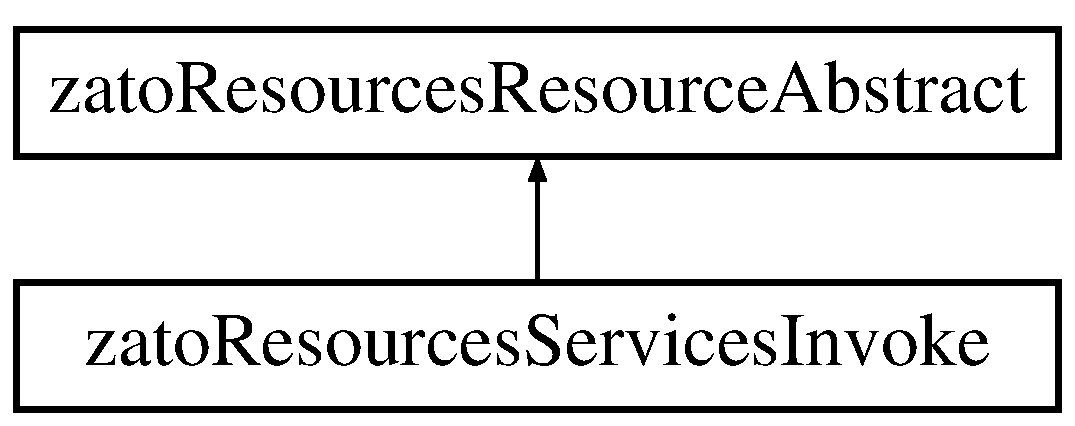
\includegraphics[height=2.000000cm]{classzato_1_1_resources_1_1_services_1_1_invoke}
\end{center}
\end{figure}
\subsection*{Public Member Functions}
\begin{DoxyCompactItemize}
\item 
\hypertarget{classzato_1_1_resources_1_1_services_1_1_invoke_ad5864994c11ba455cb85fa17767d3133}{}{\bfseries execute} (\$params=array())\label{classzato_1_1_resources_1_1_services_1_1_invoke_ad5864994c11ba455cb85fa17767d3133}

\end{DoxyCompactItemize}
\subsection*{Static Public Member Functions}
\begin{DoxyCompactItemize}
\item 
\hypertarget{classzato_1_1_resources_1_1_services_1_1_invoke_ab115b6a4302042a8482ebfa2cbf26111}{}static {\bfseries ex} (\$params=array())\label{classzato_1_1_resources_1_1_services_1_1_invoke_ab115b6a4302042a8482ebfa2cbf26111}

\end{DoxyCompactItemize}
\subsection*{Protected Attributes}
\begin{DoxyCompactItemize}
\item 
\hyperlink{classzato_1_1_resources_1_1_services_1_1_invoke_a0b74d2abc0d3878703c6da02b2db6972}{\$resource\+Name} = \textquotesingle{}zato.\+service.\+invoke\textquotesingle{}
\end{DoxyCompactItemize}


\subsection{Member Data Documentation}
\hypertarget{classzato_1_1_resources_1_1_services_1_1_invoke_a0b74d2abc0d3878703c6da02b2db6972}{}\index{zato\+::\+Resources\+::\+Services\+::\+Invoke@{zato\+::\+Resources\+::\+Services\+::\+Invoke}!\$resource\+Name@{\$resource\+Name}}
\index{\$resource\+Name@{\$resource\+Name}!zato\+::\+Resources\+::\+Services\+::\+Invoke@{zato\+::\+Resources\+::\+Services\+::\+Invoke}}
\subsubsection[{\$resource\+Name}]{\setlength{\rightskip}{0pt plus 5cm}zato\textbackslash{}\+Resources\textbackslash{}\+Services\textbackslash{}\+Invoke\+::\$resource\+Name = \textquotesingle{}zato.\+service.\+invoke\textquotesingle{}\hspace{0.3cm}{\ttfamily [protected]}}\label{classzato_1_1_resources_1_1_services_1_1_invoke_a0b74d2abc0d3878703c6da02b2db6972}
\{\} 

The documentation for this class was generated from the following file\+:\begin{DoxyCompactItemize}
\item 
src/zato/\+Resources/\+Services/Invoke.\+php\end{DoxyCompactItemize}

\hypertarget{classzato_1_1_resources_1_1_core_1_1_ping}{}\section{zato\textbackslash{}Resources\textbackslash{}Core\textbackslash{}Ping Class Reference}
\label{classzato_1_1_resources_1_1_core_1_1_ping}\index{zato\textbackslash{}\+Resources\textbackslash{}\+Core\textbackslash{}\+Ping@{zato\textbackslash{}\+Resources\textbackslash{}\+Core\textbackslash{}\+Ping}}
Inheritance diagram for zato\textbackslash{}Resources\textbackslash{}Core\textbackslash{}Ping\+:\begin{figure}[H]
\begin{center}
\leavevmode
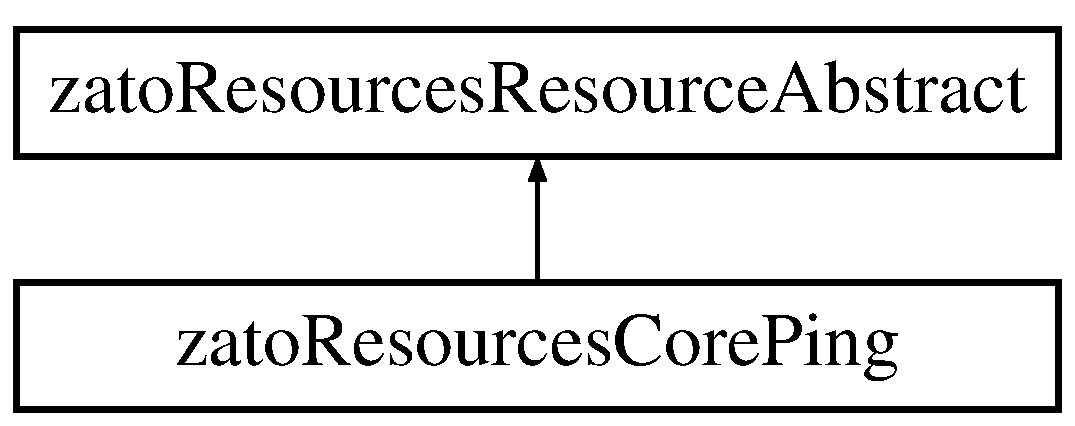
\includegraphics[height=2.000000cm]{classzato_1_1_resources_1_1_core_1_1_ping}
\end{center}
\end{figure}
\subsection*{Public Member Functions}
\begin{DoxyCompactItemize}
\item 
\hypertarget{classzato_1_1_resources_1_1_core_1_1_ping_a0a65349ad498398230002935c8cdf29d}{}{\bfseries execute} ()\label{classzato_1_1_resources_1_1_core_1_1_ping_a0a65349ad498398230002935c8cdf29d}

\end{DoxyCompactItemize}
\subsection*{Protected Attributes}
\begin{DoxyCompactItemize}
\item 
\hyperlink{classzato_1_1_resources_1_1_core_1_1_ping_ae43661c6c12c8b762537bbda5e7e2c1e}{\$resource\+Name} = \textquotesingle{}zato.\+ping\textquotesingle{}
\end{DoxyCompactItemize}


\subsection{Member Data Documentation}
\hypertarget{classzato_1_1_resources_1_1_core_1_1_ping_ae43661c6c12c8b762537bbda5e7e2c1e}{}\index{zato\+::\+Resources\+::\+Core\+::\+Ping@{zato\+::\+Resources\+::\+Core\+::\+Ping}!\$resource\+Name@{\$resource\+Name}}
\index{\$resource\+Name@{\$resource\+Name}!zato\+::\+Resources\+::\+Core\+::\+Ping@{zato\+::\+Resources\+::\+Core\+::\+Ping}}
\subsubsection[{\$resource\+Name}]{\setlength{\rightskip}{0pt plus 5cm}zato\textbackslash{}\+Resources\textbackslash{}\+Core\textbackslash{}\+Ping\+::\$resource\+Name = \textquotesingle{}zato.\+ping\textquotesingle{}\hspace{0.3cm}{\ttfamily [protected]}}\label{classzato_1_1_resources_1_1_core_1_1_ping_ae43661c6c12c8b762537bbda5e7e2c1e}
\{\} 

The documentation for this class was generated from the following file\+:\begin{DoxyCompactItemize}
\item 
src/zato/\+Resources/\+Core/Ping.\+php\end{DoxyCompactItemize}

\hypertarget{classzato_1_1_resources_1_1_resource_abstract}{}\section{zato\textbackslash{}Resources\textbackslash{}Resource\+Abstract Class Reference}
\label{classzato_1_1_resources_1_1_resource_abstract}\index{zato\textbackslash{}\+Resources\textbackslash{}\+Resource\+Abstract@{zato\textbackslash{}\+Resources\textbackslash{}\+Resource\+Abstract}}
Inheritance diagram for zato\textbackslash{}Resources\textbackslash{}Resource\+Abstract\+:\begin{figure}[H]
\begin{center}
\leavevmode
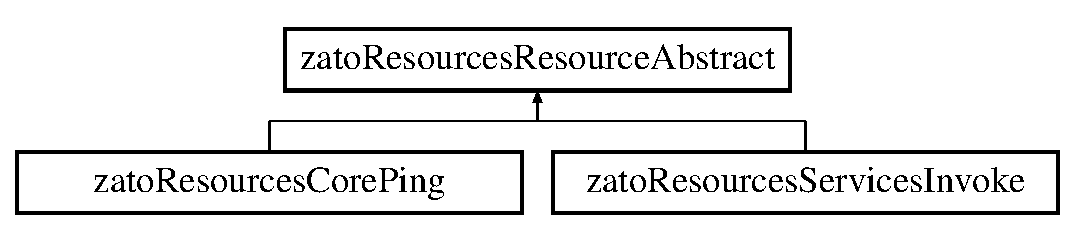
\includegraphics[height=2.000000cm]{classzato_1_1_resources_1_1_resource_abstract}
\end{center}
\end{figure}
\subsection*{Public Member Functions}
\begin{DoxyCompactItemize}
\item 
\hyperlink{classzato_1_1_resources_1_1_resource_abstract_aa98406a8a1925c090cdb54690abe8286}{\+\_\+\+\_\+construct} (\hyperlink{classzato_1_1_zato_client}{Zato\+Client} \$client)
\end{DoxyCompactItemize}
\subsection*{Protected Attributes}
\begin{DoxyCompactItemize}
\item 
\hypertarget{classzato_1_1_resources_1_1_resource_abstract_a7f7f386dbbc5dd2cc54f8b70779d5776}{}{\bfseries \$client}\label{classzato_1_1_resources_1_1_resource_abstract_a7f7f386dbbc5dd2cc54f8b70779d5776}

\end{DoxyCompactItemize}


\subsection{Constructor \& Destructor Documentation}
\hypertarget{classzato_1_1_resources_1_1_resource_abstract_aa98406a8a1925c090cdb54690abe8286}{}\index{zato\+::\+Resources\+::\+Resource\+Abstract@{zato\+::\+Resources\+::\+Resource\+Abstract}!\+\_\+\+\_\+construct@{\+\_\+\+\_\+construct}}
\index{\+\_\+\+\_\+construct@{\+\_\+\+\_\+construct}!zato\+::\+Resources\+::\+Resource\+Abstract@{zato\+::\+Resources\+::\+Resource\+Abstract}}
\subsubsection[{\+\_\+\+\_\+construct(\+Zato\+Client \$client)}]{\setlength{\rightskip}{0pt plus 5cm}zato\textbackslash{}\+Resources\textbackslash{}\+Resource\+Abstract\+::\+\_\+\+\_\+construct (
\begin{DoxyParamCaption}
\item[{{\bf Zato\+Client}}]{\$client}
\end{DoxyParamCaption}
)}\label{classzato_1_1_resources_1_1_resource_abstract_aa98406a8a1925c090cdb54690abe8286}

\begin{DoxyParams}[1]{Parameters}
Http\+Client & {\em \$client} & \\
\hline
\end{DoxyParams}


The documentation for this class was generated from the following file\+:\begin{DoxyCompactItemize}
\item 
src/zato/\+Resources/Resource\+Abstract.\+php\end{DoxyCompactItemize}

\hypertarget{classzato_1_1_zato_client}{}\section{zato\textbackslash{}Zato\+Client Class Reference}
\label{classzato_1_1_zato_client}\index{zato\textbackslash{}\+Zato\+Client@{zato\textbackslash{}\+Zato\+Client}}
\subsection*{Public Member Functions}
\begin{DoxyCompactItemize}
\item 
\hypertarget{classzato_1_1_zato_client_a1cc8c9c0397013ec5b4db5d314fd3f40}{}{\bfseries \+\_\+\+\_\+construct} (\$config=array(), \$client\+\_\+opts=array())\label{classzato_1_1_zato_client_a1cc8c9c0397013ec5b4db5d314fd3f40}

\item 
\hyperlink{classzato_1_1_zato_client_a53b3620c1606bef34ae5a63eef32f5f1}{get\+Headers} ()
\item 
\hyperlink{classzato_1_1_zato_client_ab1694e645df20117a171d3555493f11b}{get\+Api\+Url} ()
\item 
\hyperlink{classzato_1_1_zato_client_a24af3dc18befd6c3f4043b638d861e17}{get\+User\+Agent} ()
\item 
\hyperlink{classzato_1_1_zato_client_a09c7f937c1df19d0406582dc60f217ee}{set\+Debug} (\$last\+Request\+Headers, \$last\+Request\+Body, \$last\+Response\+Code, \$last\+Response\+Headers, \$last\+Response\+Error)
\item 
\hyperlink{classzato_1_1_zato_client_ae27d7f7a5200b9c2b8d179de8766e5ef}{get\+Debug} ()
\item 
\hyperlink{classzato_1_1_zato_client_a8f8b11e5ff12ce6c04b6f2c83438dd8e}{post} (\$endpoint, \$post\+Data=\mbox{[}$\,$\mbox{]})
\item 
\hyperlink{classzato_1_1_zato_client_a848f024e0c4617beec769064b0804c61}{ping} ()
\item 
\hyperlink{classzato_1_1_zato_client_aa4ee97642e8ca3b97d83a43d69f30c6c}{service\+Invoke} (\$params)
\end{DoxyCompactItemize}
\subsection*{Public Attributes}
\begin{DoxyCompactItemize}
\item 
\hypertarget{classzato_1_1_zato_client_a0ddb33d2c114aa69772dbff2c102b5e8}{}const {\bfseries V\+E\+R\+S\+I\+O\+N} = \textquotesingle{}0.\+1\textquotesingle{}\label{classzato_1_1_zato_client_a0ddb33d2c114aa69772dbff2c102b5e8}

\item 
\hypertarget{classzato_1_1_zato_client_a0f902c04331ccd1e6e6472ff474ee40e}{}{\bfseries \$guzzle}\label{classzato_1_1_zato_client_a0f902c04331ccd1e6e6472ff474ee40e}

\end{DoxyCompactItemize}
\subsection*{Protected Attributes}
\begin{DoxyCompactItemize}
\item 
\hypertarget{classzato_1_1_zato_client_a674d21f5f1f85c67108fc5d32270e2e3}{}{\bfseries \$user}\label{classzato_1_1_zato_client_a674d21f5f1f85c67108fc5d32270e2e3}

\item 
\hypertarget{classzato_1_1_zato_client_a6a60705a05ead6f984e5021e6732b679}{}{\bfseries \$pass}\label{classzato_1_1_zato_client_a6a60705a05ead6f984e5021e6732b679}

\item 
\hypertarget{classzato_1_1_zato_client_a23581082511d86f7ff4bfd95a3f7ea38}{}{\bfseries \$scheme}\label{classzato_1_1_zato_client_a23581082511d86f7ff4bfd95a3f7ea38}

\item 
\hypertarget{classzato_1_1_zato_client_aa784337aedae2c6d133b47f8e39cbb4b}{}{\bfseries \$hostname}\label{classzato_1_1_zato_client_aa784337aedae2c6d133b47f8e39cbb4b}

\item 
\hypertarget{classzato_1_1_zato_client_a22970e1fe49cbb785395be8e864b62e4}{}{\bfseries \$port}\label{classzato_1_1_zato_client_a22970e1fe49cbb785395be8e864b62e4}

\item 
\hypertarget{classzato_1_1_zato_client_a69cef41eff5d4b6672b3c991ed6ce8d3}{}{\bfseries \$api\+Url}\label{classzato_1_1_zato_client_a69cef41eff5d4b6672b3c991ed6ce8d3}

\item 
\hypertarget{classzato_1_1_zato_client_a9b87cfb04bd1f2ae050d7766fba55b79}{}{\bfseries \$debug}\label{classzato_1_1_zato_client_a9b87cfb04bd1f2ae050d7766fba55b79}

\end{DoxyCompactItemize}


\subsection{Detailed Description}
Class zato\+\_\+\+Client 

\subsection{Member Function Documentation}
\hypertarget{classzato_1_1_zato_client_ab1694e645df20117a171d3555493f11b}{}\index{zato\+::\+Zato\+Client@{zato\+::\+Zato\+Client}!get\+Api\+Url@{get\+Api\+Url}}
\index{get\+Api\+Url@{get\+Api\+Url}!zato\+::\+Zato\+Client@{zato\+::\+Zato\+Client}}
\subsubsection[{get\+Api\+Url()}]{\setlength{\rightskip}{0pt plus 5cm}zato\textbackslash{}\+Zato\+Client\+::get\+Api\+Url (
\begin{DoxyParamCaption}
{}
\end{DoxyParamCaption}
)}\label{classzato_1_1_zato_client_ab1694e645df20117a171d3555493f11b}
Returns the generated api U\+R\+L

\begin{DoxyReturn}{Returns}
string 
\end{DoxyReturn}
\hypertarget{classzato_1_1_zato_client_ae27d7f7a5200b9c2b8d179de8766e5ef}{}\index{zato\+::\+Zato\+Client@{zato\+::\+Zato\+Client}!get\+Debug@{get\+Debug}}
\index{get\+Debug@{get\+Debug}!zato\+::\+Zato\+Client@{zato\+::\+Zato\+Client}}
\subsubsection[{get\+Debug()}]{\setlength{\rightskip}{0pt plus 5cm}zato\textbackslash{}\+Zato\+Client\+::get\+Debug (
\begin{DoxyParamCaption}
{}
\end{DoxyParamCaption}
)}\label{classzato_1_1_zato_client_ae27d7f7a5200b9c2b8d179de8766e5ef}
Returns debug information from last call in an object

\begin{DoxyReturn}{Returns}
\hyperlink{classzato_1_1_debug}{Debug} 
\end{DoxyReturn}
\hypertarget{classzato_1_1_zato_client_a53b3620c1606bef34ae5a63eef32f5f1}{}\index{zato\+::\+Zato\+Client@{zato\+::\+Zato\+Client}!get\+Headers@{get\+Headers}}
\index{get\+Headers@{get\+Headers}!zato\+::\+Zato\+Client@{zato\+::\+Zato\+Client}}
\subsubsection[{get\+Headers()}]{\setlength{\rightskip}{0pt plus 5cm}zato\textbackslash{}\+Zato\+Client\+::get\+Headers (
\begin{DoxyParamCaption}
{}
\end{DoxyParamCaption}
)}\label{classzato_1_1_zato_client_a53b3620c1606bef34ae5a63eef32f5f1}
\begin{DoxyReturn}{Returns}
array 
\end{DoxyReturn}
\hypertarget{classzato_1_1_zato_client_a24af3dc18befd6c3f4043b638d861e17}{}\index{zato\+::\+Zato\+Client@{zato\+::\+Zato\+Client}!get\+User\+Agent@{get\+User\+Agent}}
\index{get\+User\+Agent@{get\+User\+Agent}!zato\+::\+Zato\+Client@{zato\+::\+Zato\+Client}}
\subsubsection[{get\+User\+Agent()}]{\setlength{\rightskip}{0pt plus 5cm}zato\textbackslash{}\+Zato\+Client\+::get\+User\+Agent (
\begin{DoxyParamCaption}
{}
\end{DoxyParamCaption}
)}\label{classzato_1_1_zato_client_a24af3dc18befd6c3f4043b638d861e17}
Return the user agent string

\begin{DoxyReturn}{Returns}
string 
\end{DoxyReturn}
\hypertarget{classzato_1_1_zato_client_a848f024e0c4617beec769064b0804c61}{}\index{zato\+::\+Zato\+Client@{zato\+::\+Zato\+Client}!ping@{ping}}
\index{ping@{ping}!zato\+::\+Zato\+Client@{zato\+::\+Zato\+Client}}
\subsubsection[{ping()}]{\setlength{\rightskip}{0pt plus 5cm}zato\textbackslash{}\+Zato\+Client\+::ping (
\begin{DoxyParamCaption}
{}
\end{DoxyParamCaption}
)}\label{classzato_1_1_zato_client_a848f024e0c4617beec769064b0804c61}
A ping service which always returns a constant string. Useful for testing clients against zato clusters.

\begin{DoxyReturn}{Returns}
std\+Class Object that has the same properties as the corresponding zato response 
\end{DoxyReturn}
\hypertarget{classzato_1_1_zato_client_a8f8b11e5ff12ce6c04b6f2c83438dd8e}{}\index{zato\+::\+Zato\+Client@{zato\+::\+Zato\+Client}!post@{post}}
\index{post@{post}!zato\+::\+Zato\+Client@{zato\+::\+Zato\+Client}}
\subsubsection[{post(\$endpoint, \$post\+Data=[])}]{\setlength{\rightskip}{0pt plus 5cm}zato\textbackslash{}\+Zato\+Client\+::post (
\begin{DoxyParamCaption}
\item[{}]{\$endpoint, }
\item[{}]{\$post\+Data = {\ttfamily \mbox{[}\mbox{]}}}
\end{DoxyParamCaption}
)}\label{classzato_1_1_zato_client_a8f8b11e5ff12ce6c04b6f2c83438dd8e}
This is a helper method to do a post request.


\begin{DoxyParams}[1]{Parameters}
string & {\em \$endpoint} & \\
\hline
array & {\em \$post\+Data} & \\
\hline
\end{DoxyParams}
\begin{DoxyReturn}{Returns}
std\+Class 
\end{DoxyReturn}

\begin{DoxyExceptions}{Exceptions}
{\em Api\+Response\+Exception} & \\
\hline
\end{DoxyExceptions}
\hypertarget{classzato_1_1_zato_client_aa4ee97642e8ca3b97d83a43d69f30c6c}{}\index{zato\+::\+Zato\+Client@{zato\+::\+Zato\+Client}!service\+Invoke@{service\+Invoke}}
\index{service\+Invoke@{service\+Invoke}!zato\+::\+Zato\+Client@{zato\+::\+Zato\+Client}}
\subsubsection[{service\+Invoke(\$params)}]{\setlength{\rightskip}{0pt plus 5cm}zato\textbackslash{}\+Zato\+Client\+::service\+Invoke (
\begin{DoxyParamCaption}
\item[{}]{\$params}
\end{DoxyParamCaption}
)}\label{classzato_1_1_zato_client_aa4ee97642e8ca3b97d83a43d69f30c6c}
Invokes a service by its I\+D or name. From the service’s viewpoint, there is no difference between being invoked directly, through a channel or if using zato.\+service.\+invoke.

If executing a service in async mode, its response will be a C\+I\+D it’s been invoked with.

Client configuration settings include the following options\+:


\begin{DoxyItemize}
\item id int Service I\+D. Either id or name must be provided.
\item name string Service name. Either id or name must be provided.
\item payload string Data to be used as input by the zato service, can be any P\+H\+P type except a resource.
\item channel string Channel the service will believe it’s being invoked over
\item data\+\_\+format string Payload’s data format (json set as default)
\item transport string Transport the service should believe it’s being invoked with
\item async boolean Whether the service should be invoked asynchronously, defaults to False
\item expiration int If using async mode, after how many seconds the message should expire, defaults to 15 seconds
\end{DoxyItemize}


\begin{DoxyParams}[1]{Parameters}
array & {\em \$params} & \\
\hline
\end{DoxyParams}
\begin{DoxyReturn}{Returns}
std\+Class Decoded payload object from service invoke 
\end{DoxyReturn}
\hypertarget{classzato_1_1_zato_client_a09c7f937c1df19d0406582dc60f217ee}{}\index{zato\+::\+Zato\+Client@{zato\+::\+Zato\+Client}!set\+Debug@{set\+Debug}}
\index{set\+Debug@{set\+Debug}!zato\+::\+Zato\+Client@{zato\+::\+Zato\+Client}}
\subsubsection[{set\+Debug(\$last\+Request\+Headers, \$last\+Request\+Body, \$last\+Response\+Code, \$last\+Response\+Headers, \$last\+Response\+Error)}]{\setlength{\rightskip}{0pt plus 5cm}zato\textbackslash{}\+Zato\+Client\+::set\+Debug (
\begin{DoxyParamCaption}
\item[{}]{\$last\+Request\+Headers, }
\item[{}]{\$last\+Request\+Body, }
\item[{}]{\$last\+Response\+Code, }
\item[{}]{\$last\+Response\+Headers, }
\item[{}]{\$last\+Response\+Error}
\end{DoxyParamCaption}
)}\label{classzato_1_1_zato_client_a09c7f937c1df19d0406582dc60f217ee}
Set debug information as an object


\begin{DoxyParams}[1]{Parameters}
mixed & {\em \$last\+Request\+Headers} & \\
\hline
mixed & {\em \$last\+Request\+Body} & \\
\hline
mixed & {\em \$last\+Response\+Code} & \\
\hline
string & {\em \$last\+Response\+Headers} & \\
\hline
mixed & {\em \$last\+Response\+Error} & \\
\hline
\end{DoxyParams}


The documentation for this class was generated from the following file\+:\begin{DoxyCompactItemize}
\item 
src/zato/Zato\+Client.\+php\end{DoxyCompactItemize}

%--- End generated contents ---

% Index
\backmatter
\newpage
\phantomsection
\clearemptydoublepage
\addcontentsline{toc}{chapter}{Index}
\printindex

\end{document}
